Description of the problem ($\FP+\CC+\MA+\BW$).

\subsection{Dynamic programming on trees}

Intro to dynamic programming on trees with subtree decomposition.
Introduce binarization as way of dealing with trees of larger arity.
Mention correctness requirements: substructure optimality and overlapping subproblems.

\subsection{Introduction to our algorithm}

We will want to go through all VM placements, for each of those do greedy matching and choose the cheapest.

Solution for subtree - how it can look like? It is ``partial matching''. Some matched VMs and chunks, but also some chunks transported out of subtree or some VMs/slots that will have chunks transported into from outside. So we charge already those incomplete matchings.

Cost charging model - two edges. Recursive formula for calculating the cost.
Recursive formula for cost with bandwidth. 

\subsection{Algorithm}

TODO: hosting multiple VMs in the same node

List all needed functions like distance, counter of number of chunks in subtree.

Present the pseudocode, with base cases, aggregate function.

Tell how to go back through the array to reconstruct the actual placements. ``Following path of minimas''.
Note that it computationally intensive, and we can trade it for memory - we can remember the best placement.

\subsection{Algorithm correctness}
\subsubsection{Optimality of greedy matching}

For general complete bipartite graphs the matching constructed by greedily choosing the cheapest edge can be arbitrarily bad.
However, in case of very specific graph, where weights are induced by distance in a tree, this strategy produces optimal solution.
By using properties of the tree, we will show following lemma:

\begin{lemma}
  Given fixed positions of VMs, the local greedy perfect matching of chunks to VMs inclines minimal cost among all possible perfect matchings.
\end{lemma}

\begin{proof}
Proof by contradiction. Let's assume that there exists matching of cost lower than cost of $G$. Let's take cheapest such matching and call it $H$.

Let's find smallest subtree $S$ where partial matching of $G$ has different cost than partial matching of $H$. It means that in both left and right subtree we did local matching (do we need this sentence?). It means that non-local decision was made in this subtree (perhaps hoping for savings higher?). Then there exist two such two such matched pairs in $H$ that shares an edge (one pair is transporting chunk up, the second one is transporting chunk down). Then we can create matching $H'$ that uncrosses those edges (does the local matching on them) and is cheaper than $H$. Contradiction.


\end{proof}

It means basically that in every subtree we can only have more costly solution. Perhaps there exist cleaner way of proving that.

\subsubsection{Substructure optimality.}

What is our substructure? It is unfinished matching. Show that we can build optimal matching out of those unfinished ones. Here we need to
consider different number of VMs to choose best composition.

Basically, it is the correctness proof of our strategy. You have to use optimality of greedy matching here.

\subsubsection{Bandwidth correctness.}

\begin{lemma}
  If algorithm returns solution $\Sol$ of cost $\neq \infty$, then in $\Sol$ no link exceeds its capacity limit.
  \end{lemma}

\begin{lemma}
An instance of $\Problem$ is infeasible iff. algorithm returns $\infty$.
\end{lemma}
\begin{proof}
  ($\rightarrow$)

  ($\leftarrow$)
  \end{proof}


\subsection{Running time and memory consumption analysis}

\begin{figure}
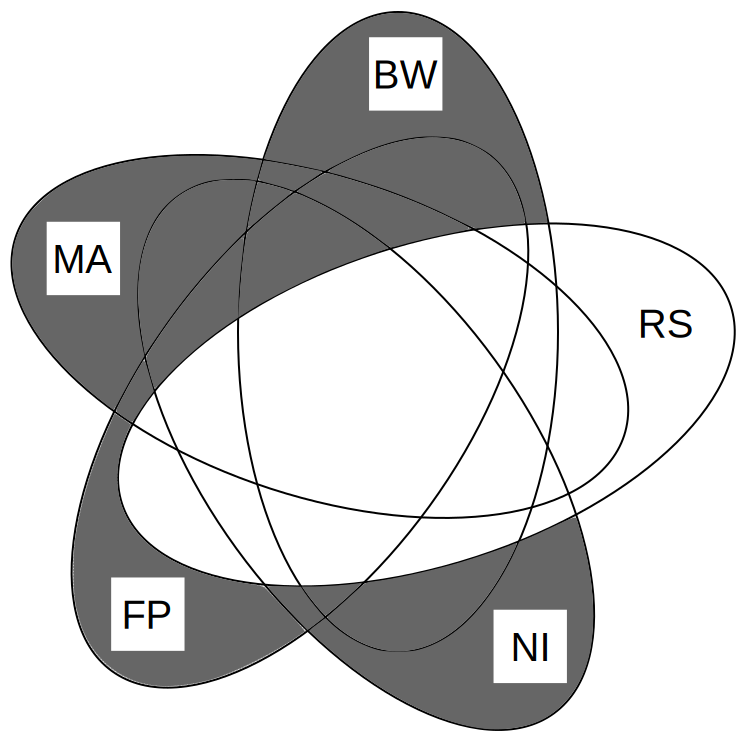
\includegraphics[width=\columnwidth]{figs/venn_dp.pdf}
\caption{Property combinations which can be solved by our dynamic prorgramming 
appraoch.}
\label{fig:venn_dp}
\end{figure}

\carlo{Figure~\ref{fig:venn_dp} shows illustrates which problem 
combiantions can be solved by the presented dynamic programming approach.}
